\documentclass[11pt,conference,a4paper,twocolumns,romanappendices]{IEEEtran}
\usepackage[utf8]{inputenc}
\usepackage[english]{babel}
\usepackage{verbatim}
\usepackage{graphicx}
\usepackage{wrapfig}
\author{Lucas Kummer, Samuel Sedlmeir, Lucas Colantuono, Shanan Lynch}

\title{Recommendations guiding taxi traffic by heatmaps}
\date{\today}

\author{
\IEEEauthorblockN{Lucas Kummer}
\IEEEauthorblockA{INSA Lyon\\
lucas.kummer@insa-lyon.fr}
\and
\IEEEauthorblockN{Samuel Sedlmeir}
\IEEEauthorblockA{INSA Lyon\\
S.Sedlmeir@campus.lmu.de}
\and
\IEEEauthorblockN{Lucas Colantuono}
\IEEEauthorblockA{INSA Lyon \\
lucas.colantuono@insa-lyon.fr}
\and
\IEEEauthorblockN{Shanan Lynch}
\IEEEauthorblockA{INSA Lyon\\
shanan.lynch@insa-lyon.fr}
}

\begin{document}

\maketitle

\tableofcontents
\newpage

\begin{abstract}
With a growing interest in Internet of Things (IoT) trace information in recent years, data mining has proven itself to be an excellent method for detecting fascinating human behaviours.
Deployed in the right manner these behaviours could not only affect the way individuals act but influence the demeanour of sizeable companies.
This paper mainly focuses on analysing IoT traces of taxis in the area of Shanghai and using methods such as heatmaps and trip analysis. Using these methods to recommend times of deployment and what areas to deploy taxi drivers.
\end{abstract}

\section{Introduction}
The ability to data mine information gathered from IoT traces has attracted a lot of attention throughout recent years. The information that can be collected via IoT devices used in house appliances, phones and vehicles are endless.
Our focus on vehicles and more specifically taxis gives us the opportunity to change or even improve the daily routine of taxi drivers, taxi reliability, and taxi companies.
Articles mentioned in the related work section (\ref{sec:relatedWork}) of this paper display the tremendous potentials of taxi IoT traces that can and already have been explored.
We decided to concentrate on patterns of human behaviour that would affect clients, taxi drivers, and profit for taxi companies. Furthermore we had to assure ourselves that the information gathered by the IoT trace was consistent. Following this analysis we used methods such as heat mapping and taxi routes analysis to determine what we would recommend to taxi drivers and companies. In conclusion we found that there were too many taxis in the north city of Shanghai compared to the client demand. Inversely the demand in the center of the city was more than the north. In conclusion this would mean that we would recommend that the taxis not in demand in the north should move towards the center of the city.
\label{sec:Introduction}

\section{Related work}
There are several different articles, that analyse the same or similar datasets and compute different models and metrics. \\
The first article is written by chinese researchers who analysed the Taxi GPS traces from Shanghai in order to develop a model that helps to understand the needs of vehicular ad hoc networks for example. Therefore the authors computed several metrics, e.g. the turn probability at all the road crossings, implemented a map-matching algorithm and considered macro- and microscopic travel patterns. Their so called "META" model shows a higher accuracy than all other models at this time. \cite{meta} \\
A different approach is presented by American researchers in their article. They haven't used GPS traces, but collected traces from users on a campus via WiFi routers, where the users' smartphones are automatically registered. Thereby they are able to develop a model, which makes it possible for them to detect a hierarchy of the different access points and cluster them. These clusters are being analysed in terms of the size distribution as well as inter- and intra-cluster travel patterns. \cite{wlan} \\
Another article about the taxi data set from Shanghai aimed to find an algorithm, that allows fair route sharing for every competing taxi driver. One of its goals is to not lose efficiency and to have driving cost per customer as low as possible, so that it offers advantages for the driver and the customer equally. This requires a complex evaluation algorithm that considers several priniciples which are respected by the assignment mechanism. \cite{scram} \\
In contrast to other public transports, taxi drivers plan their own routes once they drop off a passenger. Some articles are about recommended routes that aim to save time for taxi drivers and potential passengers. \\
In general, there are three ways to develop recommender systems. The first one is content based which means suggesting items that are similar to those a user liked in the past. The second way is based on recommendations computed according to the preferences of other users similar to the target user. The third one is an hybrid solution. \\
T-Finder provides taxi drivers with detailed information not only about the route, but also about parking spaces. \cite{tf} The goal of the work described in this article is to propose an approach to detect parking spaces based on a large number of GPS trajectories generated by taxis, where the parking spaces stand for the locations where taxi drivers usually wait for passengers with their taxis parked. T-Finder enhances the passenger recommender by estimating the waiting time on a specified nearby road segment in addition to calculating the probability of finding a vacant taxi. \\
LCP \cite{eff} uses the same method as T-Finder \cite{tf} to extract the representative small areas from the trajectories. The goal of the LCP route recommendation algorithm is to find an energy-efficient mobile recommender system by exploiting the energy-efficient driving patterns extracted from the location traces of Taxi drivers. This system has the ability to recommend a sequence of potential pick-up points for a driver in a way such that the potential travel distance before getting a customer is minimized. \\
Identifying user interests and providing personalized suggestions, the different recommender systems address and collect information to reduce the spent time of passengers and taxi drivers. Recommender systems \cite{tow} presents an overview of the field of recommender systems and describes the current generation of recommendation methods and various ways to extend the capabilities of recommender systems as well. This article concluded that recommender systems made significant progress over the last decade when numerous content-based, collaborative and hybrid methods were proposed and several "industrial-strength" systems have been developed. \\
Recommender systems by mining large-scale \cite{min1,min2} data develop a smart recommendation system based on extracted patterns and data from studies focused of large-scale trace data collected by a probe taxi. Large-scale trace data provide us with opportunities to extract useful transportation patterns and utilize these patterns to improve efficiency.
\label{sec:relatedWork}

\section{Data consistency}
The first task is to check and improve the consistency of the provided data, so that we are able to compute our heatmaps accurately, which we achieved by developing an R script.\\
At the beginning we have to filter all impossible values of the variables we're operating on. For example, our script removes all entries with a negative speed value or timestamps outside of the interval in which these data have been collected.  Apparently the trace files only contain consistent data sets as our script has not detected and removed a single error. \\
Furthermore, there are two more types of errors that have to be considered: Checking the geographical consistency and filtering gaps in the traces.

\subsection{Geographical consistency}
In the next step we analysed several statistical metrics concerning the speed variable which showed that there is a wide spectrum of different values, with some outliers bigger than 200 km/h, which does not make any sense in a city centre and is probably an error. That's why we decided to cut off all the entries with a speed higher than three times the interquartile range. As you can see in figure \ref{fig:speed_before} the speed distribution is skewed right with a single maximum. That justifies our decision, because we don't lose relevant data entries, when we choose our cut-off speed value. On the other hand, just performing a coordinate cut is not sufficient: it changes the speed distribution slightly, e.g. we lost some data entries on the street towards one of the airports by removing all the points with a speed higher than 80 km/h. However, it does not remove all error entries. \\

\begin{figure}[h]
\centering
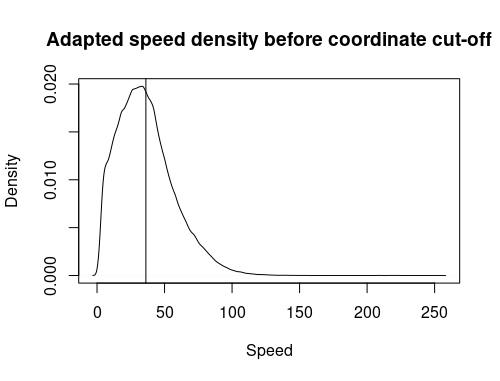
\includegraphics[scale=0.6]{density_before.png}
\caption{\label{fig:speed_before}Adapted speed distribution without zero values, but before coordinate filtering}
\end{figure}

The data still has to be filtered by the coordinates. As we decided to focus on the city centre, we only keep those entries in our dataset that have a longitude between 121.38 and 121.57 and a latitude between 31.15 and 31.32. In figure \ref{fig:borders} you can see our chosen borders on a map with a random sample of 100.000 points. \\

\begin{figure}[h]
\centering
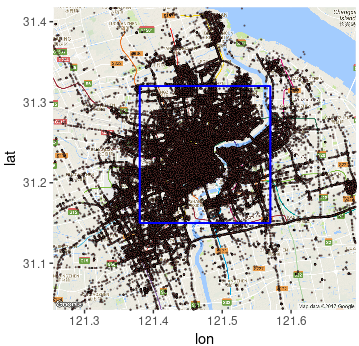
\includegraphics[scale=0.9]{borders.png}
\caption{\label{fig:borders}Borders of the city center}
\end{figure}

After restricting the data to this area, we observed a change in the distribution of the speed values as well: In general, the mean slightly decreases, in this case from 36.95 km/h to 34.06 km/h, whilst the median is increasing more significantly, as the amount of datasets with a speed higher than the median that we remove (in this case) comes up to almost 30 percent of all datasets. There is also a big difference when we look at the standard deviation which falls from 21.37 to 19.3. As we have a right skewed distribution, we eliminate higher values with this procedure, which is the result of the fact that some streets outside of the city center don't have a low speed limit and make it necessary to perform this cut-off: for example it decreases the amount of datasets with a speed higher than 80km/h by more than one half, see figure \ref{fig:speed_after}. \\

\begin{figure}[h]
\centering
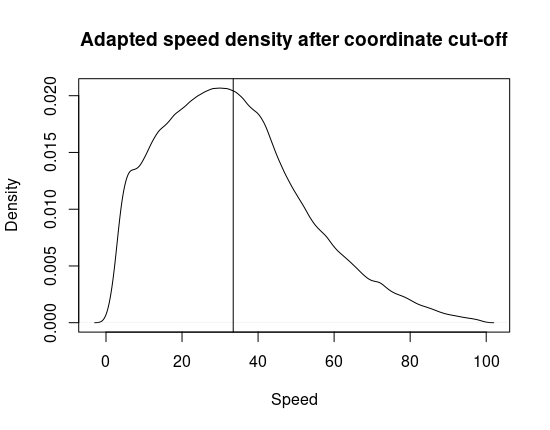
\includegraphics[scale=0.6]{density_after.png}
\caption{\label{fig:speed_after}Adapted speed distribution without zero values, after coordinate filtering}
\end{figure}

\subsection{Gap filtering}
After this procedure we are already able to plot a schematic map of Shanghai, although our dataset still contains data to be filtered. We search for those taxi traces with a time gap between two data entries. This gap could either be a result of a data transmission error or an indicator for the beginning of a new taxi trip.\\
\begin{figure}[h]
\centering
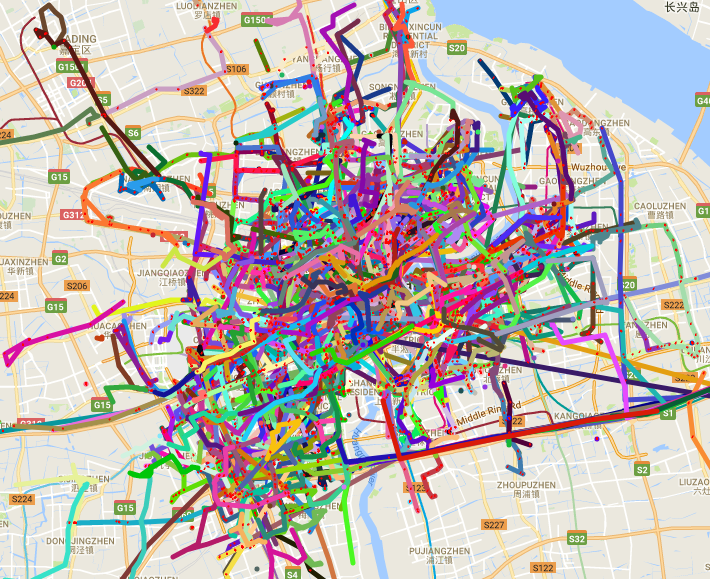
\includegraphics[scale=0.35]{plotalltrips.png}
\caption{\label{fig:plotalltrips}All calculated trips}
\end{figure}
To define these trips we had to choose a time gap that was appropriate for this data. We defined a trip by the absolute value of a time gap between two data. If it is bigger than 600 seconds, it gets separated and becomes a new trip.\\
As you can see in figure \ref{fig:timegap}, the mean value is around 25 minutes per gap in this case, while most of the gaps are shorter than 20 minutes. \\
\begin{figure}[h]
\centering
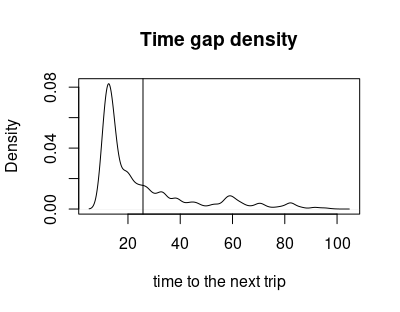
\includegraphics[scale=0.75]{timegap.png}
\caption{\label{fig:timegap}The time-gap distribution}
\end{figure}
The reason we chose this time range was because for future analyses of these trips this time range would keep our results consistent and accurate. Each of the trips would be given random colours to discern one from another if we decided to plot all of these trips like in the example given. \\

\section{Geographical Analysis: Taxi spotting versus client pickup}
The previously treated data can now be used to plot a row of heatmaps. Therefore we can vary several parameters in order to affect the appearance and its content.\\
In order to make sense of the vast amount of data, we had to read and structure it. We used Python and R to read out and sort it to our preferences. Especially the Python package "gmplot" \cite{gmplot} helped us plotting heatmaps and trips on the well known Google Maps platform. Combined with our programmed scripts, we were able to create multiple maps adapted to our liking. You can find a link to our Github Repository in the References. \cite{github-IoTTrace} \\
\subsection{Heatmap appearance parameters}
As appearance parameters we can define the center position of the heatmap which will be positioned in the very center of Shanghai. Apart from that we can define the threshold, radius, gradient, opacity and a dissipating factor. The threshold is a value that defines how many data points are required at a certain spot in order to be displayed as a different coloured circle whose size is defined by the radius. The gradient parameter controls the colour gradient, whereas the opacity variable is responsible for the degree of transparency the circles will show. The dissipating factor controls whether the data is scattering as soon as one zooms into the map.
Amongst those parameters, we focus on the radius parameter, as it has the biggest influence. It highly depends on the size of the heatmap: the further we zoom in, the smaller the radius must become, otherwise we will display huge circles on a high-level-zoom map, which contains hardly any information. As we only compute a certain restricted area, we can focus on three zoom levels, which we have to find an optimal radius value for. In general one can say, that for each level we zoom in, we should double the radius in order to keep hotspots at the same points and with the same size. A reasonable value for the radius at zoom level 11 would be 15 pixels, so 30 pixels for level 12 or 60 pixels for level 13 deliver reasonable results as well. Figures \ref{fig:zoom1} and \ref{fig:zoom2} show the negative extremes: A too big radius leads to a large and strongly connected hotspot, whereas hardly any hotspots can be found when using a radius too small.

\begin{figure}[h]
\centering
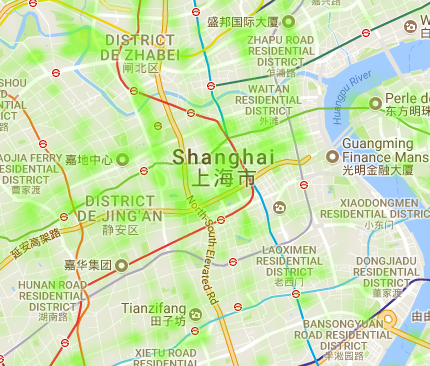
\includegraphics[scale=0.45]{zoom_too_low.png}
\caption{\label{fig:zoom1}Heatmap with a too low radius}
\end{figure}

\begin{figure}[h]
\centering
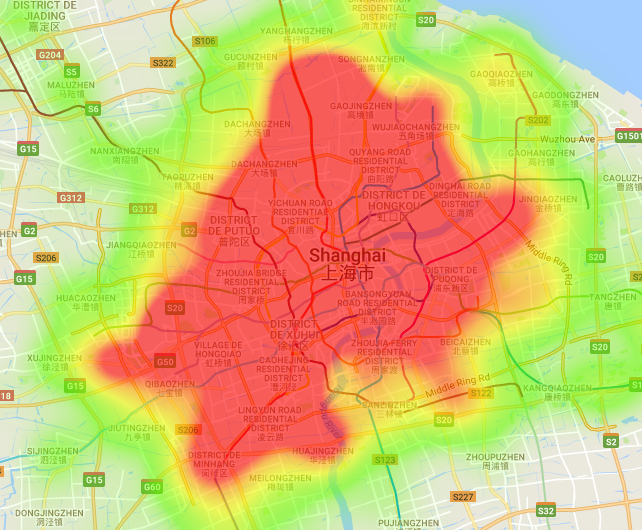
\includegraphics[scale=0.3]{zoom_too_high.png}
\caption{\label{fig:zoom2}Heatmap with a too high radius}
\end{figure}

\subsection{Heatmap content parameters}
Even more important than the appearance parameters are the parameters of the data to be displayed.
In order to not influence our observed results by sampling, we decided to process only whole files at a single time. Therefore, we adapted our algorithm.
After sampling we can make use of different parameters to either plot all data or just those with or without a passenger.
A splitting of all available data into several time slots is useful as well - in order to observe different patterns or preferred districts of the taxis.
As you can see in figure \ref{fig:allPass3to6} it is simply visible: Between 3 and 6 a.m. there is a high density in the northern center, whereas between 3 and 6 p.m. the taxis a more concentrated in the very center of Shanghai and is not that strongly scattered all over the map.

\begin{figure}
\begin{center}
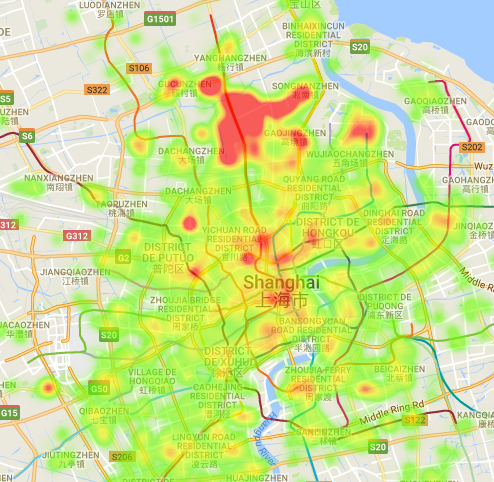
\includegraphics[width=.3\textwidth]{3to6.png}
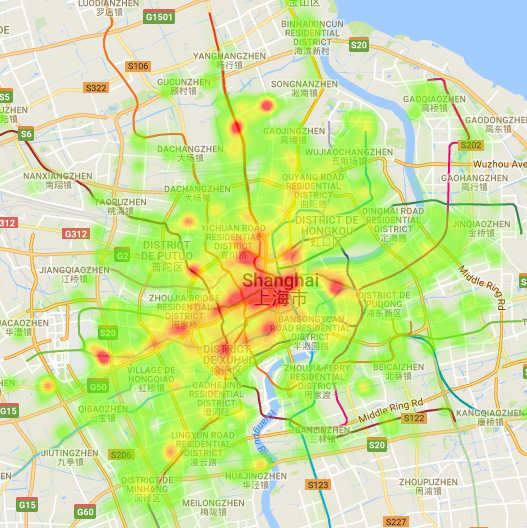
\includegraphics[width=.3\textwidth]{15to18.png}
\end{center}
\caption{\label{fig:allPass3to6}Heatmap of all taxis between 3-6 a.m. in comparison with a Heatmap of all taxis between 3-6 p.m.}
\end{figure}

\subsection{Timeslots and Division}

In order to find a suitable time window and the perfect timeslot between different heatmaps it is necessary to compare all time slots to each other instead of simply guessing a random timeslot. We started with a range of one hour and therefore created 24 different heatmaps. Furthermore we generated numerous heatmaps for two, three, six and twelve hour slots, as well as a heatmap of the whole dataset which represents 24 hours. Those tests were concluded on taxi drivers that currently drive with passengers as well as those that drive without them.\\
In Figure \ref{fig:w pass 0-3 1h&3h}, \ref{fig:w pass 0-12 3h&6h}, and \ref{fig:w pass 0-12 6h&12h} we can see heatmaps of taxis with passengers. They are splitted up in 1, 3, 6 and 12 hour timeslots, always starting at midnight. The nearest or rather neighbouring timeslots are put into relation to each other in each figure.\\
Figures \ref{fig:wo pass 0-3 1h&3h}, \ref{fig:wo pass 0-12 3h&6h}, and \ref{fig:wo pass 0-12 6h&12h} show the same patterns but use data of taxis without passengers.
All named heatmaps follow the directions left to right primarily and then top to down. \\
When taking a look at Figure \ref{fig:w pass 0-3 1h&3h} and \ref{fig:wo pass 0-3 1h&3h}, each of which shows three one hour slots compared to a 3 hour slot, you can make out that between the one hour slots there is hardly any difference. Taxis with passengers are slowly moving from the center of Shanghai to the north of the city and the other way round for taxis without passengers, but this is also easy to make out on the three hour time slots.\\
If we go on and analyse given three hour slots to the six hour slots (Figure \ref{fig:w pass 0-12 3h&6h} and \ref{fig:wo pass 0-12 3h&6h}) we come to the conclusion that a six hour slot is too imprecise, because it is hard to make out specific movements of taxis, an observation that is true for all 12 hour slots as well. Therefore we concluded that we should focus on heatmaps divided into three hour slots, in order to make out how and where taxis move around the city of Shanghai.

\begin{figure}
\begin{center}
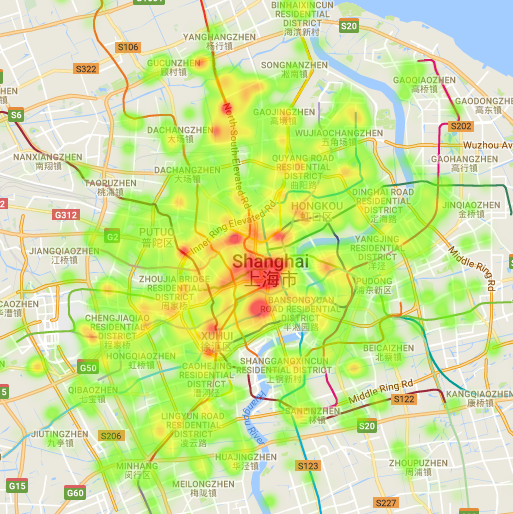
\includegraphics[width=.2\textwidth]{../heatmaps/1_slots/pass_1h/heatmap_mediumbibig_pass_0-1.PNG}
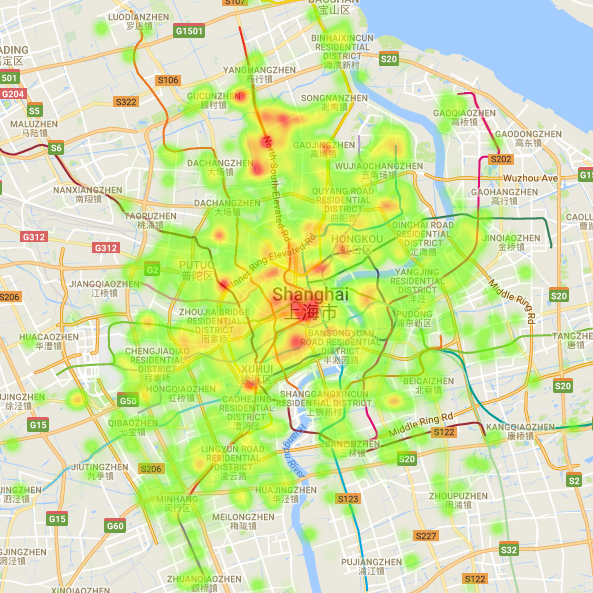
\includegraphics[width=.2\textwidth]{../heatmaps/1_slots/pass_1h/heatmap_mediumbibig_pass_1-2.PNG}
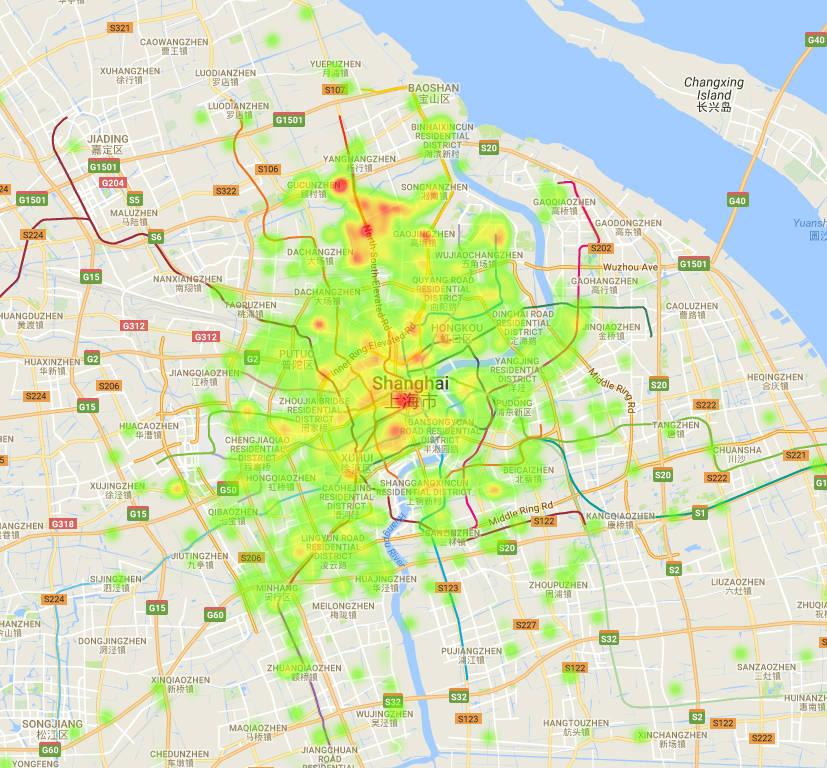
\includegraphics[width=.2\textwidth]{../heatmaps/1_slots/pass_1h/heatmap_mediumbibig_pass_2-3.PNG}
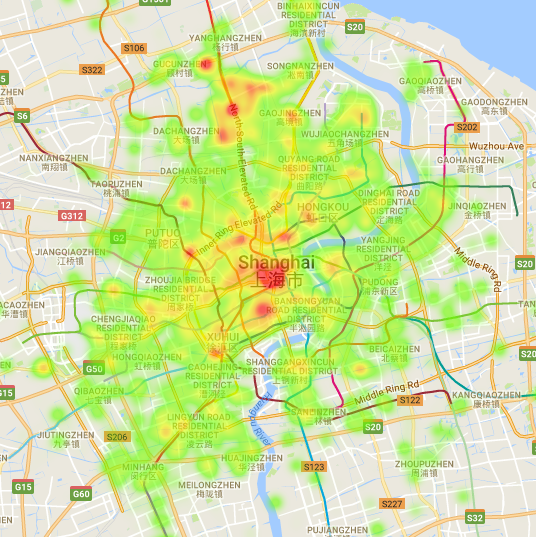
\includegraphics[width=.2\textwidth]{../heatmaps/3_slots/pass_3h/heatmap_mediumbibig_pass_0-3.PNG}
\end{center}
\caption{\label{fig:w pass 0-3 1h&3h}Heatmaps with passengers; left top: 0-1 am, right top: 1-2 am, left bottom: 2-3 am, right bottom: 0-3 a.m.}
\end{figure}

\begin{figure}
\begin{center}
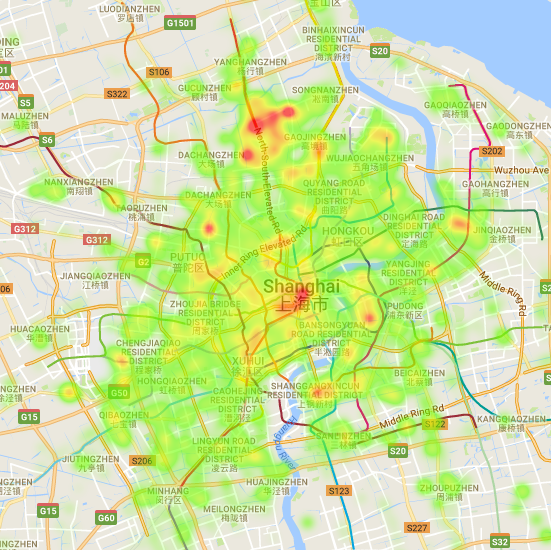
\includegraphics[width=.2\textwidth]{../heatmaps/1_slots/no_pass_1h/heatmap_mediumbibig_nopass_0-1.PNG}
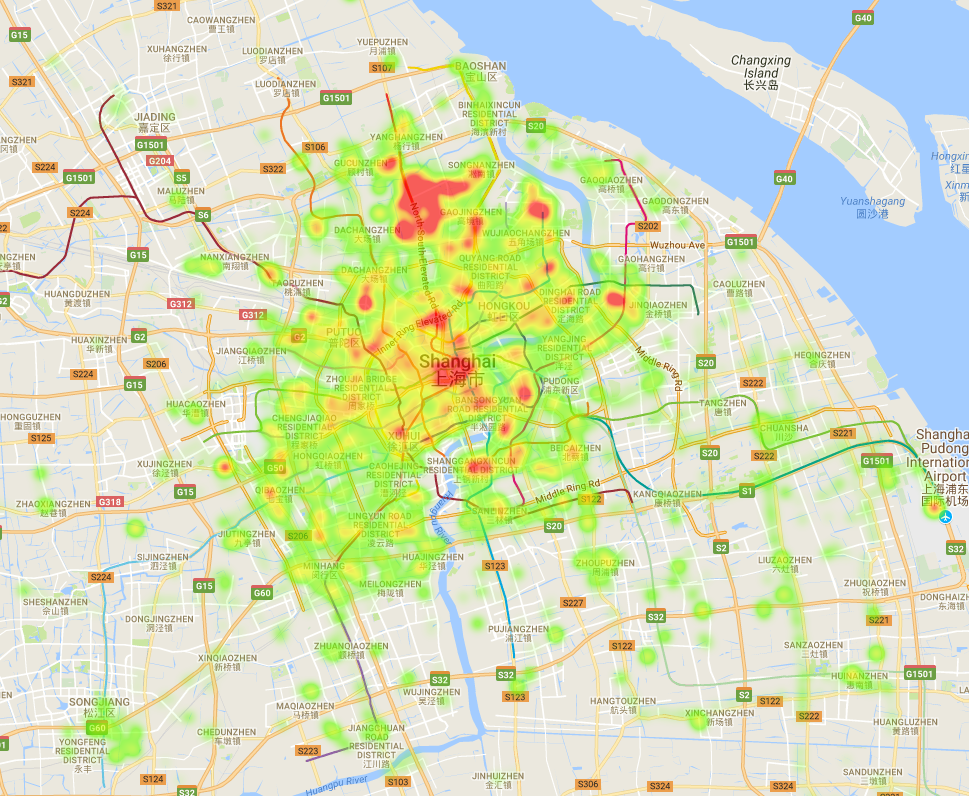
\includegraphics[width=.2\textwidth]{../heatmaps/1_slots/no_pass_1h/heatmap_mediumbibig_nopass_1-2.PNG}
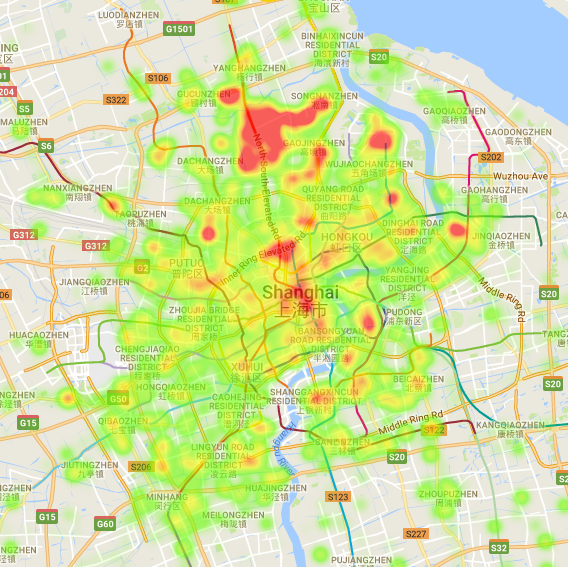
\includegraphics[width=.2\textwidth]{../heatmaps/1_slots/no_pass_1h/heatmap_mediumbibig_nopass_2-3.PNG}
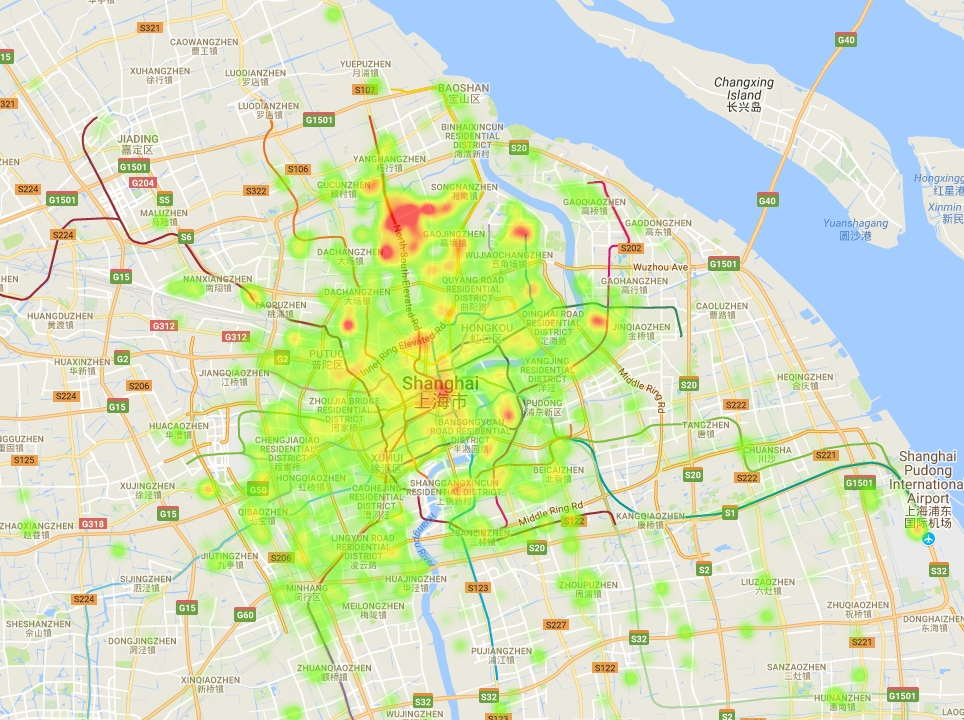
\includegraphics[width=.2\textwidth]{../heatmaps/3_slots/nopass_3h/heatmap_mediumbibig_nopass_0-3.PNG}
\end{center}
\caption{\label{fig:wo pass 0-3 1h&3h}Heatmaps without passengers; left top: 0-1 a.m., right top: 1-2 a.m., left bottom: 2-3 a.m., right bottom: 0-3 a.m.}
\end{figure}

 \begin{figure}
 \begin{center}
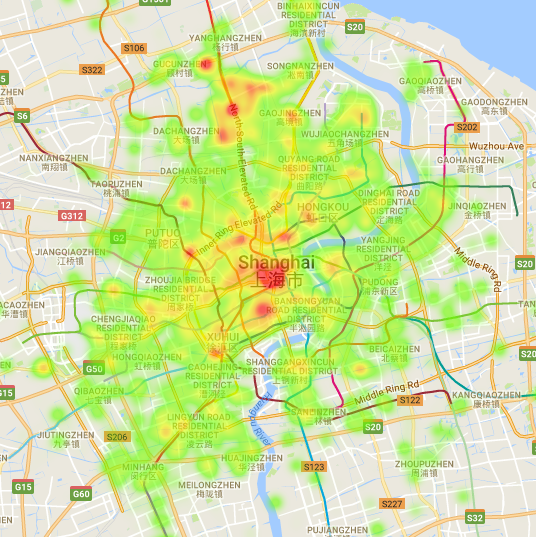
\includegraphics[width=.2\textwidth]{../heatmaps/3_slots/pass_3h/heatmap_mediumbibig_pass_0-3.PNG}
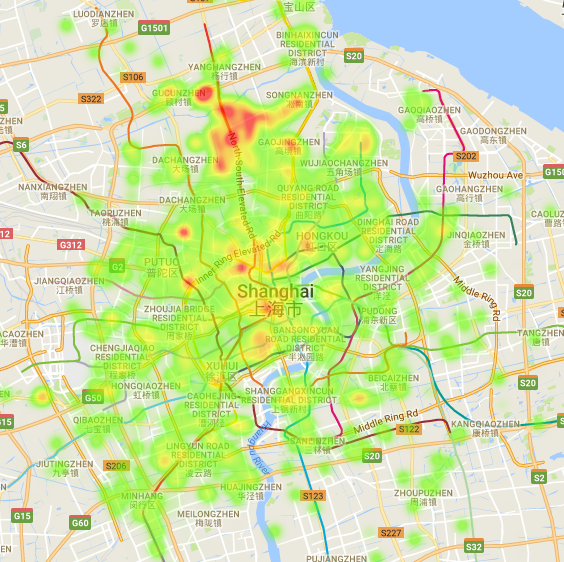
\includegraphics[width=.2\textwidth]{../heatmaps/3_slots/pass_3h/heatmap_mediumbibig_pass_3-6.PNG}
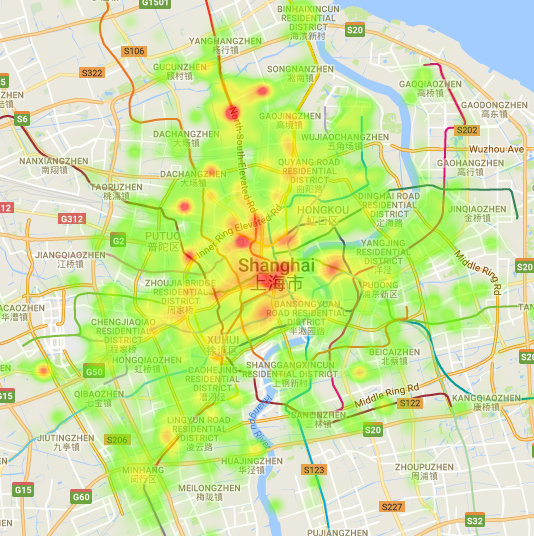
\includegraphics[width=.2\textwidth]{../heatmaps/3_slots/pass_3h/heatmap_mediumbibig_pass_6-9.PNG}
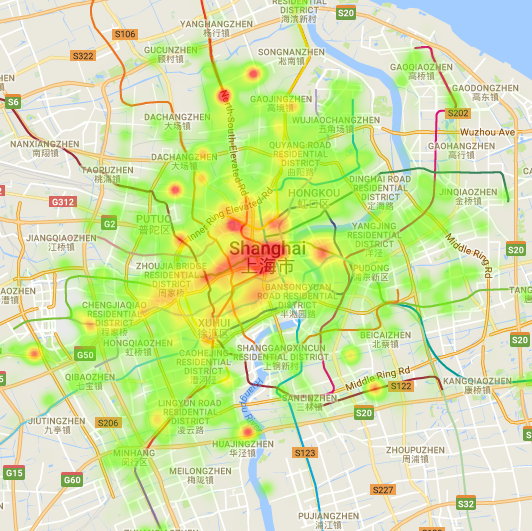
\includegraphics[width=.2\textwidth]{../heatmaps/3_slots/pass_3h/heatmap_mediumbibig_pass_9-12.PNG}
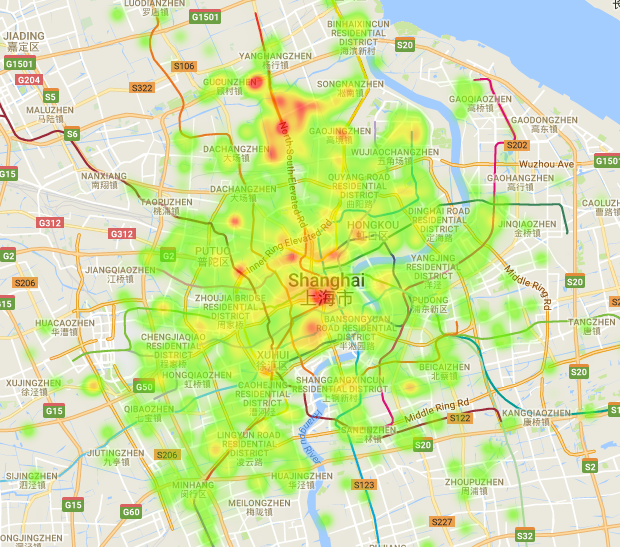
\includegraphics[width=.2\textwidth]{../heatmaps/6h_slots/0-to-6_with-pass.png}
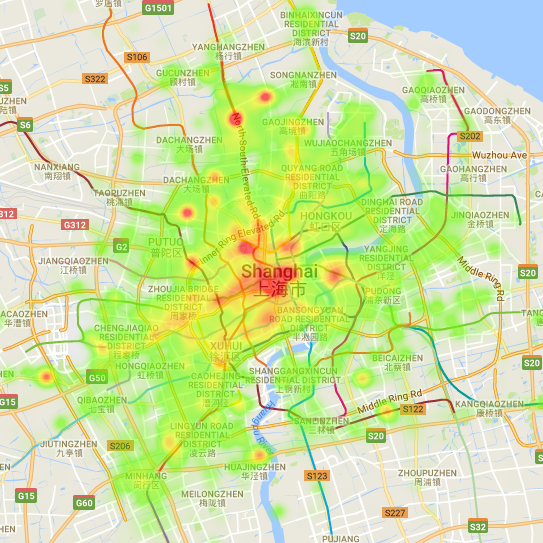
\includegraphics[width=.2\textwidth]{../heatmaps/6h_slots/6-to-12_with-pass.png}
\end{center}
\caption{\label{fig:w pass 0-12 3h&6h}Heatmaps with passengers: left top: 0-3 a.m., right top: 3-6 a.m., left center: 6-9 a.m., right center: 9-12 a.m., left bottom: 0-6 a.m., right bottom: 6-12 a.m.}
\end{figure}

 \begin{figure}
 \begin{center}
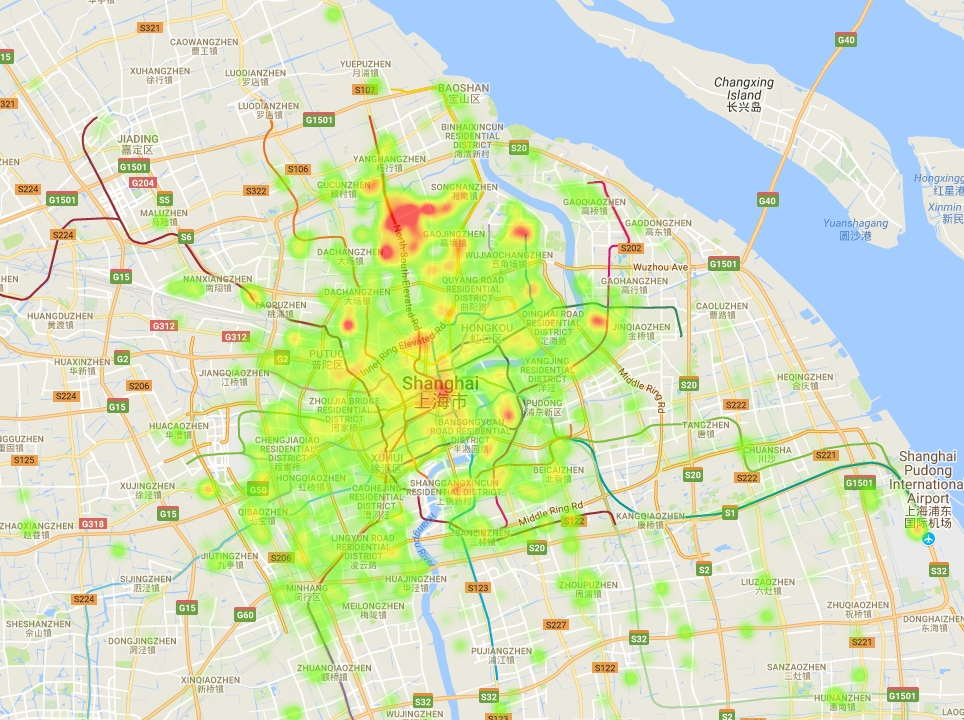
\includegraphics[width=.2\textwidth]{../heatmaps/3_slots/nopass_3h/heatmap_mediumbibig_nopass_0-3.PNG}
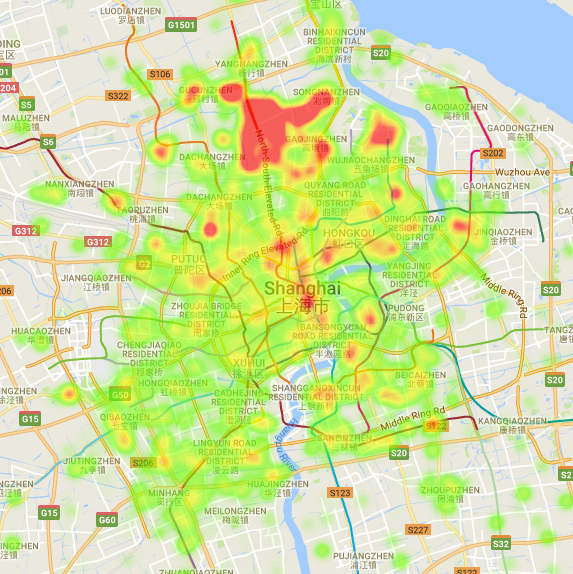
\includegraphics[width=.2\textwidth]{../heatmaps/3_slots/nopass_3h/heatmap_mediumbibig_nopass_3-6.PNG}
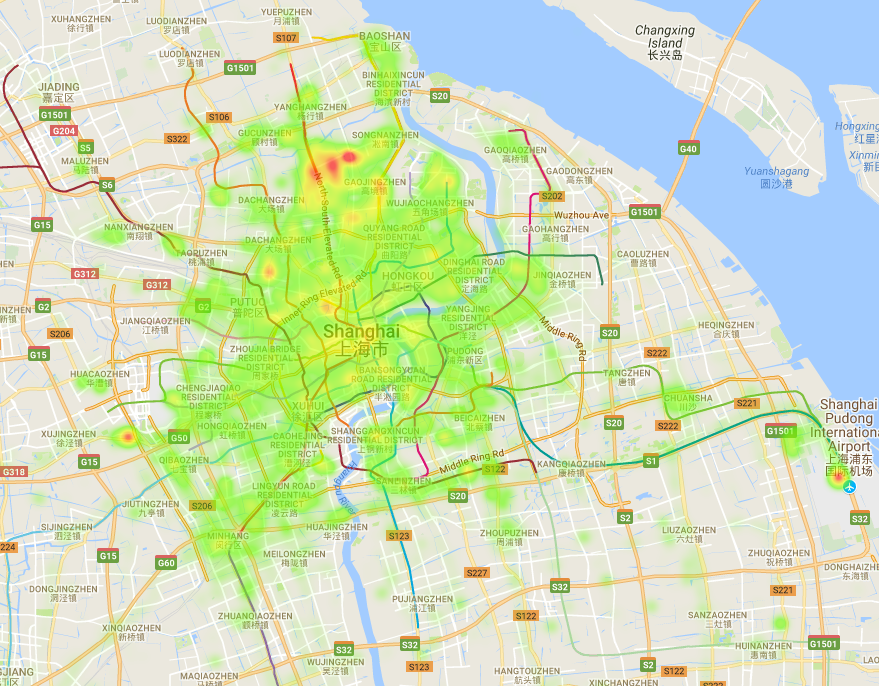
\includegraphics[width=.2\textwidth]{../heatmaps/3_slots/nopass_3h/heatmap_mediumbibig_nopass_6-9.PNG}
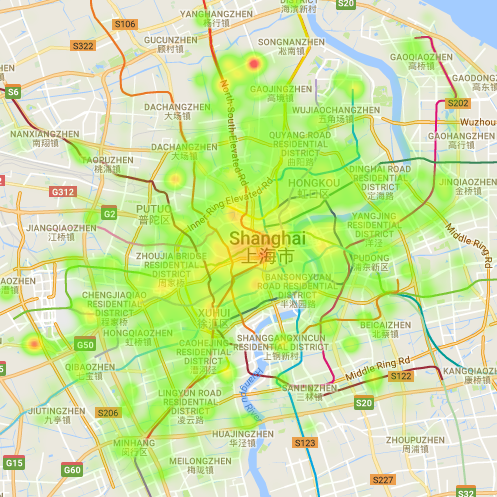
\includegraphics[width=.2\textwidth]{../heatmaps/3_slots/nopass_3h/heatmap_mediumbibig_nopass_9-12.PNG}
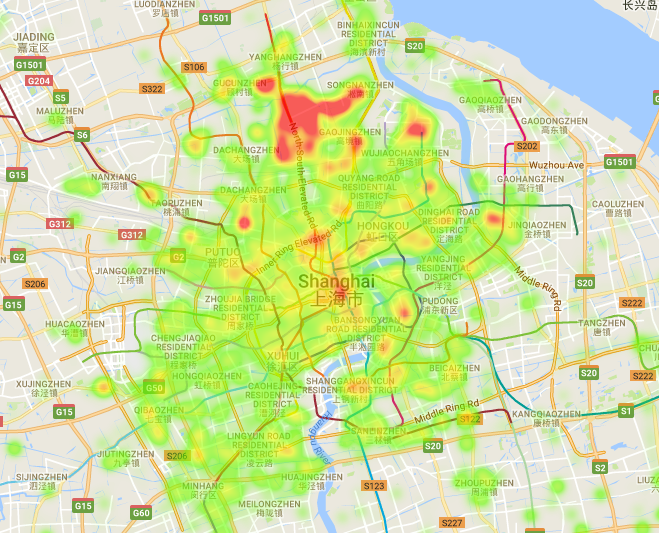
\includegraphics[width=.2\textwidth]{../heatmaps/6h_slots/0-to-6_without-pass.png}
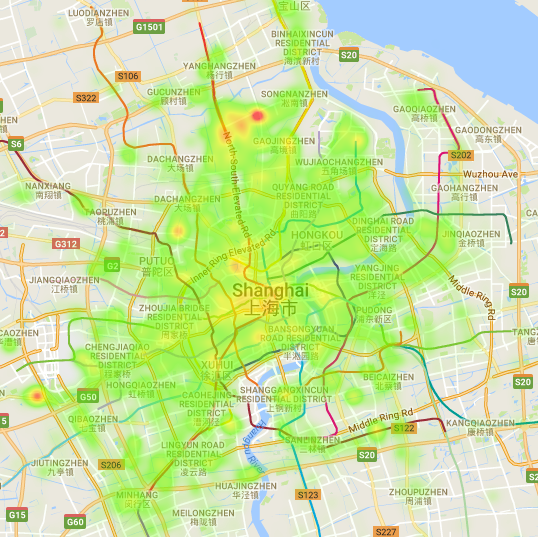
\includegraphics[width=.2\textwidth]{../heatmaps/6h_slots/6-to-12_without-pass.png}
\end{center}
\caption{\label{fig:wo pass 0-12 3h&6h}Heatmaps without passengers: left top: 0-3 a.m., right top: 3-6 a.m., left center: 6-9 a.m., right center: 9-12 a.m., left bottom: 0-6 a.m., right bottom: 6-12 a.m.}
\end{figure}

 \begin{figure}
 \begin{center}
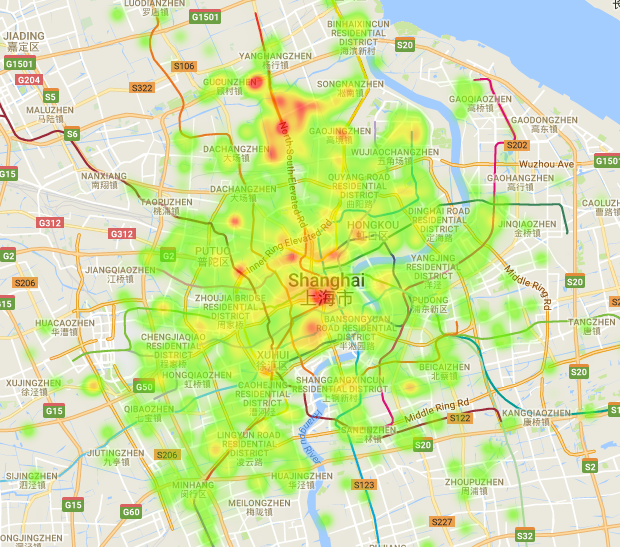
\includegraphics[width=.2\textwidth]{../heatmaps/6h_slots/0-to-6_with-pass.png}
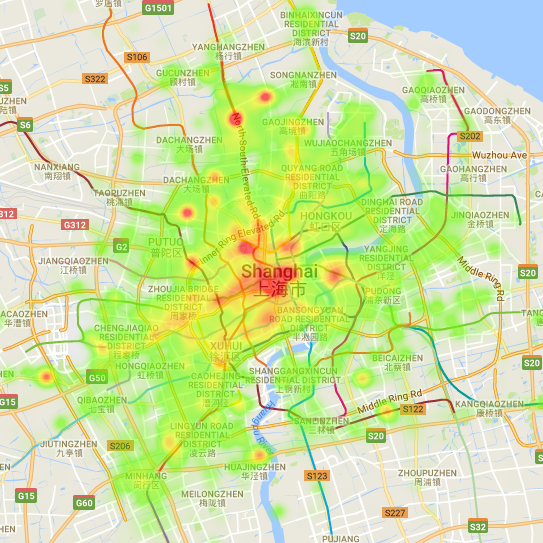
\includegraphics[width=.2\textwidth]{../heatmaps/6h_slots/6-to-12_with-pass.png}
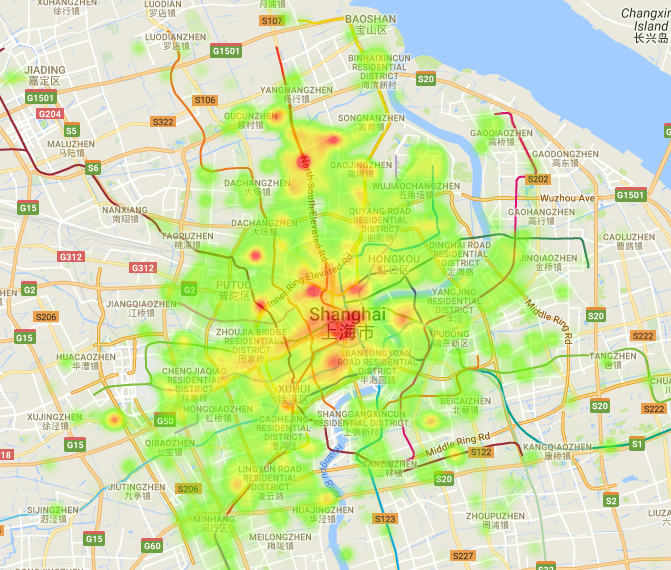
\includegraphics[width=.2\textwidth]{../heatmaps/12h_slots/0-to-12_with-pass.png}
\end{center}
\caption{\label{fig:w pass 0-12 6h&12h}Heatmaps with passengers; left top 0-6 a.m., right top: 6-12 a.m., right bottom: 0-12a.m.}
\end{figure}

 \begin{figure}
 \begin{center}
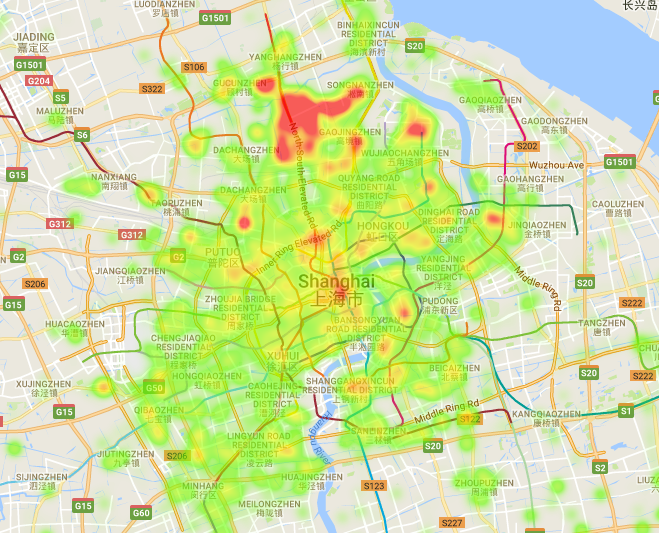
\includegraphics[width=.2\textwidth]{../heatmaps/6h_slots/0-to-6_without-pass.png}
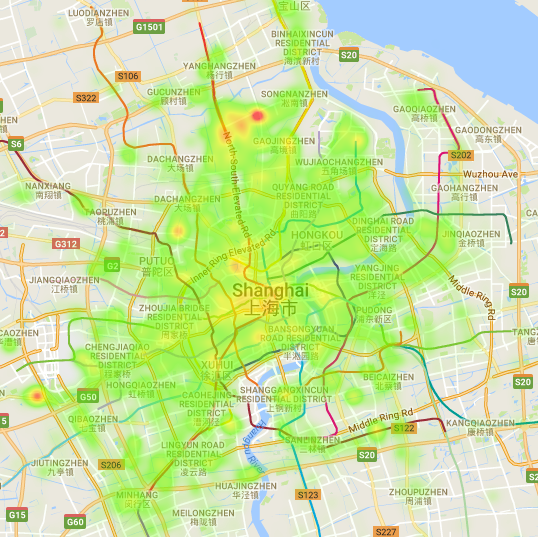
\includegraphics[width=.2\textwidth]{../heatmaps/6h_slots/6-to-12_without-pass.png}
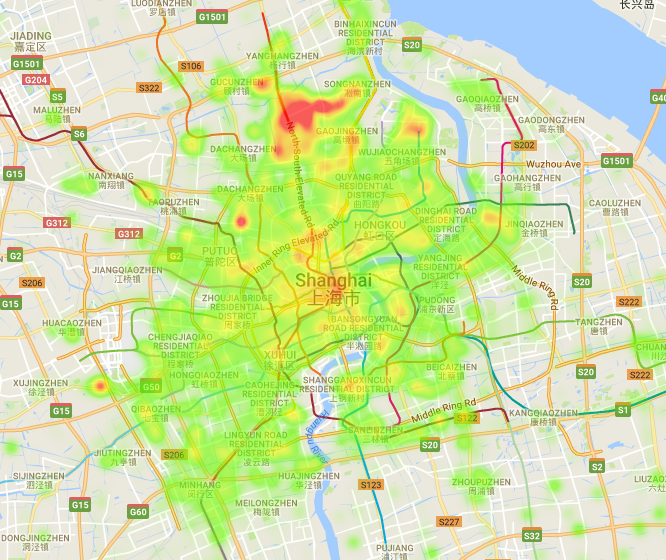
\includegraphics[width=.2\textwidth]{../heatmaps/12h_slots/0-to-12_without-pass.png}
\end{center}
\caption{\label{fig:wo pass 0-12 6h&12h}Heatmaps without passengers; left top 0-6 a.m., right top: 6-12 a.m., right bottom: 0-12a.m.}
\end{figure}

\subsection{Observable Patterns}
By comparing those different heatmaps, we can find several different behavioural patterns. \\
For example taxi traffic could be improved by trying to minimize the difference in the heatmaps with and without passengers from 0 to 3 a.m.: Whilst there are a lot of spare taxis in the north of the city, the highest density of trips is located directly in the center. \\
Two other interesting observations concern the amount of taxis in and out of use. \\
First, the density and thereby the amount of taxis without a passenger decreases significantly from the second last to the last 3h interval, whilst the amount of taxis in use even increases slightly. \\
Second, a good time to start working for a taxi driver is for example around 6 a.m., as the density of unused taxis strongly decreases, after it has been pretty high before. \\
Considering all trips, we can also gain information about the taxis in service. \\
For example, the area where most of them are located is definitely smaller after 9 a.m. than before, which might be because of a previous movement of a significant amount of people towards the city center. \\

\section{Conclusion}
As described in this paper, we got a good overview of how taxis in Shanghai behave during the day. We compared different heatmaps which are the visual representation of the taxis' density. This representation refers to the amount of taxis on a particular area of the city center. The warmer the color, the more taxis in the same area. \\
We mentioned in the section about observable patterns that after determining the best time interval, it is possible to find several different behaviours based on the time of day and the the taxi occupied condition (whether taxi is with or without passengers). \\
We discovered that there was an underestimation of the taxi demand in the center and maybe an overestimation in the north between 0 and 3 a.m., which should be improved by moving the taxis towards the center and removing then from service eventually. \\
Furthermore, available taxis are used more efficiently in the interval from 9 p.m. to 12 p.m. than in the time slot before, as waiting times decrease and the passengers per taxi ratio rises. \\
In general, we can use the heatmaps very well to detect where money can be saved by better spreading the taxis over the different time intervals. For example a lot of drivers could be moved from the time slot from 3 to 6 a.m. to the one from 12 to 3 p.m. in order to offer an highly available service, independent of the time of the day. \\
In order to customize and create heatmaps more easily, future work will be needed to create an interface where data can be filtered by criteria like whether the taxi transports passengers, an unique identifier for each taxi, date, speed, position and time. We can plan to provide real data to our work in the future, in order to detect the places that are heavily populated and used so that we can suggest some measures to improve the traffic flow in real time. Taking into consideration these cases, we will be able to validate the effectiveness of the system. \\
Furthermore, future work will can define some metrics in order to detect 'friendly' taxis, for example by working hours and proximity, which can be achieved by scaling our heatmaps' code. Therefore we can define a short distance when taxis are unoccupied at the same moment. After that, we will get the taxis that are connected by these behavioural patterns. \\
Finally, to optimize the taxi business and save time for for both the drivers and the customers, we propose the following recommendations: a reasonable start of the working time for a taxi driver, specific areas to pick up a client taking into consideration the time of day, and to add more parking places or taxi stations separated from but close to the highly demanded areas in order to improve the traffic.

\newpage

\bibliographystyle{IEEEtran}
\bibliography{biblio}
\end{document}
